\documentclass{article}
\usepackage{fullpage}
\usepackage{indentfirst}
\usepackage{amsmath}
\usepackage{amsfonts}
\usepackage{amssymb}
\usepackage{array}
\usepackage{tipa}
\usepackage{tikz}
\usepackage{tikz-qtree}
\usetikzlibrary{matrix, arrows, automata}
\usepackage{natbib}
\usepackage{gb4e}
\noautomath
\newcommand{\Y}{$\checkmark$}
\newcommand{\R}{$\Rightarrow$}
\newcommand\myeq{\mathrel{\stackrel{\makebox[0pt]{\mbox{\normalfont\tiny def}}}{=}}}
\newcommand{\ap}{\approx}
\title{Neutralization in Shanghai and Zhangping}
\author{Chris Oakden}
\begin{document}
\maketitle
Our formalization of tone sandhi as I/O mapping transductions can also accommodate cases of sandhi which neutralize underlying contrast. Interestingly, it is possible to conceive of many of these cases as procedurally similar to assimilation (via spreading) and dissimilation (via feature-changing). We illustrate with examples from Shanghai, a northern Wu dialect and Zhangping, a Min dialect. \par
\section{Shanghai}
\citet{Chen2000} points toward the well-known case of Shanghai \citep{Xuetal1981, ZeeMaddieson1980, SelkirkShen1990, Duanmu1991}  as an example of neutralization. Within the domain of a lexical compound, all non-initial tones delete, and the contour of the first syllable spreads over its entirety. Consider two disyllabic forms [ma.m\textipa{O}] `buy a cat' and [ma.m\textipa{O}] `buy a hat'; Chen conceptualizes neutralization here as a case of deletion of all non-initial tones followed by spreading.
\begin{center}
\begin{tabular}[t]{lll}
\textipa{ma} & \textipa{mO} & `buy a cat' \\
LH & HM & base tones \\
LH & . & Deletion\\
L. & H & Spread
\end{tabular}
\hspace{1cm}
\begin{tabular}[t]{lll}
\textipa{ma} & \textipa{mO} & `buy a hat' \\
LH & LM & base tones \\
LH & . & Deletion\\
L. & H & Spread
\end{tabular}
\end{center}
In Shanghai, the tonal contrast between morphemes [m\textipa{O}$^{\textnormal{HM}}$] `cat' and [m\textipa{O}$^{\textnormal{LM}}$] `hat' is \emph{neutralized} in non-domain-initial position. \par
This generalization extends to non-binary domains. As \citet{Yip1980} notes (citing \citet{ZeeMaddieson1980} and \citet{Sherard1972}), in lexical compounds of three or more syllables, all non-initial tones delete, the leftmost tone of the first syllable associates to the first syllable, with its rightmost tone spreading to the edge of the domain.
\begin{center}
\begin{tabular}[t]{llllll}
\textipa{s1} & \textipa{sang} & \textipa{c1} & `bastard' \\
HL & HL & LH & base tones \\
HL & . & . & Deletion\\
H. & L & L & Spread\\
\end{tabular}
\hspace{1cm}
\begin{tabular}[t]{llllll}
\textipa{s1} & \textipa{ka} & \textipa{dha} & \textipa{c\oe} & `world war' \\
HL & LH & LH & LH & base tones \\
HL & . & . & . & Deletion\\
H. & L & L & L & Spread\\
\end{tabular}
\end{center}
Defining a logical transduction of neutralization in Shanghai lexical compounds proceeds in a similar manner as other spreading processes; the tones which do not surface are `deleted' in the definition of the unary relations over terminal tonal nodes, and `spreading' is achieved in the definition of dominance ($\delta(x)\ap y$). As was the case with contour spread in Zhenjiang, we generate the elements which spread in an additional copy set (thereby formalizing spread and tier conflation as one mapping). This means that the size of the copy set increases linearly with the size of the compound domain. In addition, previous analyses do not explicitly discuss \emph{register} spread in this process, however it is reasonable to assume that domain-wide spread is uniform across terminal tonal elements and their registers. If the rightmost tone of an initial low-registered syllable is [l] (or conventionally, [L]), it is assumed that [L] spreads across an entire domain, even to lexically high-registered non-initial syllables. For that reason, we also spread register (generated in some copy set) to non-initial syllables. We define a transduction below for the process in a trisyllabic domain. Note that since syllable and tone root `T' nodes remain undisturbed throughout the process, their definitions are omitted here (assume that any unary relation not explicitly defined in copy sets 2 and above is set to $\mathtt{False}$).
\begin{equation}
\begin{aligned}
P^{1}_{c}(x)&\myeq P_{c}(x)\land first(x) & P^{2}_{c}(x)&\myeq P_{c}(x)\land first(x) & P^{3}_{c}(x)&\myeq P_{c}(x)\land first(x) \\
P^{1}_{+u}(x)&\myeq P_{+u}(x)\land first(x) & P^{2}_{+u}(x)&\myeq P_{+u}(x)\land first(x) & P^{3}_{+u}(x)&\myeq P_{+u}(x)\land first(x) \\
P^{1}_{-u}(x)&\myeq P_{-u}(x)\land first(x) & P^{2}_{-u}(x)&\myeq P_{-u}(x)\land first(x) & P^{3}_{-u}(x)&\myeq P_{-u}(x)\land first(x) \\
P^{1}_{h}(x)&\myeq P_{h}(x)\land first(x) & P^{2}_{h}(x)&\myeq P_{h}(x)\land first(\delta(x))\land & P^{3}_{h}(x)&\myeq P_{h}(x)\land first(\delta(x))\land \\
&& &\quad\,\, \neg first(\delta(succ(x))) & &\quad\,\, \neg first(\delta(succ(x)))\\
P^{1}_{l}(x)&\myeq P_{l}(x)\land first(x) & P^{2}_{l}(x)&\myeq P_{l}(x)\land first(\delta(x))\land & P^{3}_{l}(x)&\myeq P_{l}(x)\land first(\delta(x))\land \\
&& &\quad\,\, \neg first(\delta(succ(x))) & &\quad\,\, \neg first(\delta(succ(x)))\\
\end{aligned}
\end{equation}
These definitions guarantee a few things. First, they generate the relevant tonal information from the first syllable only in the first copy set (recall that syllables and `T' roots are fully-specified in this copy set). Crucially, only the \emph{first} terminal tonal tier node is defined in the first copy set. This will be dominated by its corresponding `c' node. In all subsequent copy sets, the non-initial tone dominated by the first syllable's `c' node (i.e. the second tonal terminal) is generated, either [l] or [h], along with register and `c' nodes from the same syllable. These elements will `spread' to the remaining non-initial syllables in the domain, one per copy set, left to right, via the definition of domination below (association is omitted as it remains constant between input and output). 
\begin{equation}
\begin{aligned}
\delta^{1,1}(x)\ap y&\myeq \big(P_{r}(x)\land P_{T}(y)\land first(x,y)\big)\,\lor \\
&\quad\,\,\big(P_{c}(x)\land P_{T}(y)\land first(x,y)\big)\,\lor \\
&\quad\,\,\big(P_{t}(x)\land P_{c}(y)\land first(x,y)\big)\,\lor \\
\delta^{2,1}(x)\ap y &\myeq \big(P_{r}(x)\land P_{T}(y)\land first(x) \land \delta(succ(x))\ap y \big)\,\lor \\
&\quad\,\,\big(P_{c}(x)\land P_{T}(y)\land first(x)\land \delta(succ(x))\ap y \big) \\
\delta^{2,2}(x)\ap y &\myeq P_{t}(x)\land P_{c}(y)\land first(\delta(x))\land\neg first(\delta(succ(x)))\land first(y)\land\delta(x)\ap y \\
\delta^{3,1}(x)\ap y &\myeq \big(P_{r}(x)\land P_{T}(y)\land first(x) \land \delta(succ(succ(x)))\ap y \big)\,\lor \\
&\quad\,\,\big(P_{c}(x)\land P_{T}(y)\land first(x)\land \delta(succ(succ(x)))\ap y \big) \\
\delta^{3,3}(x)\ap y &\myeq P_{t}(x)\land P_{c}(y)\land first(\delta(x))\land\neg first(\delta(succ(x)))\land first(y)\land\delta(x)\ap y \\
\end{aligned}
\end{equation}
Other logically possible dominance relations between copy sets ($\delta^{1,2}$, $\delta^{1,3}$, $\delta^{2,3}$, $\delta^{3,2}$) are set to $\mathtt{False}$. These definitions will map an input structure to an output structure consistent with the reported empirical generalizations. The initial tone associates to the first syllable, while the second tone in the first syllable (along with its register) associates to all non-initial syllables.\footnote{This transduction accommodates contour tones, but what about level tones? Shanghai is an interesting case in this regard. \citet{Chen2000} notes the controversy surrounding the inventory of lexical tones in the language (saying that it can be narrowed down to two), but describes it as a five-tone language, four of which are contours: /HL, MH, LH, LMq, Hq/. There is some hesitation to discuss cases for which checked tones are domain-initial (see for example \citet{Zhang2007}) given the often unruly behavior of checked tones in general. I leave this discussion for future work and admit that while this transduction generalizes most of the possible tonal combinations in Shanghai lexical compounds, it is as yet incomplete.}\par
Linear order over tiers proceeds through the first copy set for syllables and roots, and between copy sets for all other elements. As before, successor relations between elements which do not conform to the domain-wide spreading generalization (e.g. $succ^{1,3}$, $succ^{2,1}$, $succ^{2,2}$, $succ^{3,2}$, $succ^{3,1}$) are set to $\mathtt{False}$.
\begin{equation}
\begin{aligned}
succ^{1,1}(x)\ap y&\myeq \big(P_{\sigma}(x,y)\land succ(x)\ap y\big)\lor \big(P_{T}(x,y)\land succ(x)\ap y\big)\\
succ^{1,2}(x)\ap y&\myeq \big(P_{r}(x,y)\land x\ap y\big) \lor \big(P_{c}(x,y)\land x\ap y\big) \lor \\
&\quad\,\,\big(P_{t}(x,y)\land first(x)\land first(\delta(y))\land \neg first(\delta(succ(y)))\big) \\
succ^{2,3}(x)\ap y&\myeq \big(P_{r}(x,y)\land x\ap y\big)\lor\big(P_{c}(x,y)\land x\ap y\big)\lor\big(P_{t}(x,y)\land x\ap y\big) \\
succ^{3,3}(x)\ap y&\myeq \big(P_{r}(x,y)\land x\ap y\big)\lor\big(P_{c}(x,y)\land x\ap y\big)\lor\big(P_{t}(x,y)\land x\ap y\big) \\
\end{aligned}
\end{equation}
Applied to the input /HL.HL.LH/, the output of the transduction is as follows. Successor relations between copy sets are contained in a separate graph for clarity.\footnote{What about an alternative analysis which formalizes this type of neutralization as a feature-changing operation instead of spread and tier conflation? While this analysis may appear simpler, there are reasons to believe it is not preferable to the current analysis. Assuming a definition of unary relations over terminal tonal nodes such that all non-initial terminals are the same (I haven't yet devised a way to do this in QF), there is the issue of the resulting structure. On non-initial underlying contours, the result would be two tonal nodes dominated by the same `c' which share the same feature.\\
\begin{tikzpicture}[sibling distance =15pt]
\tikzset{level distance = 20pt}
\Tree [.c [.l ] [.l ] ];
\end{tikzpicture}
\hspace{1cm}
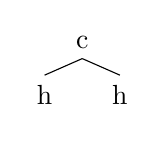
\begin{tikzpicture}[sibling distance =15pt]
\tikzset{level distance = 20pt}
\Tree [.c [.h ] [.h ] ];
\end{tikzpicture}\\
 Neither Bao nor Yip assume this structure for level tones, and it is ostensibly an OCP violation. I may discuss this further elsewhere in the QP, but for now I leave it for future work, as it will take us too far afield.}
\begin{center}
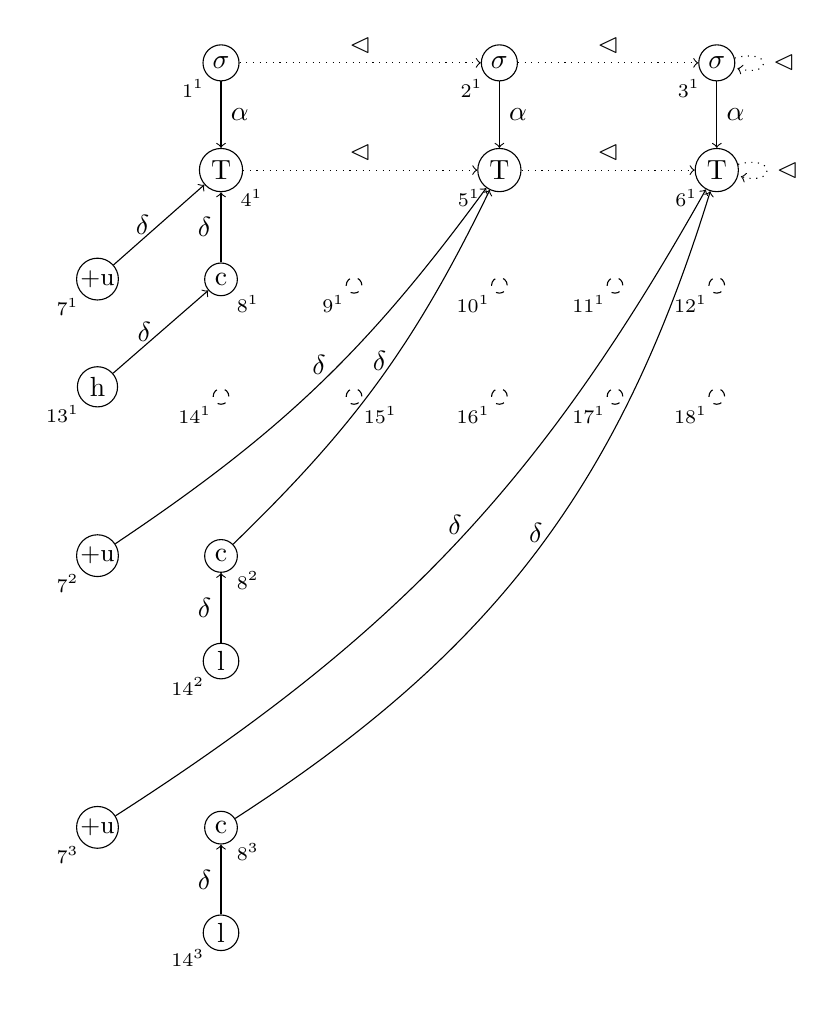
\begin{tikzpicture} [baseline = (y1.base)]
\matrix (m) [matrix of nodes, column sep = 1.5em, row sep = 1.5em]{
& \node[draw,circle, inner sep =2pt, label ={[label distance = -3pt] below left:\scriptsize$1^1$}](x1){$\sigma$}; & &  \node[draw,circle, inner sep =2pt, label ={[label distance = -3pt] below left:\scriptsize$2^1$}](x2){$\sigma$}; & &  \node[draw,circle, inner sep =2pt, label ={[label distance = -3pt] below left:\scriptsize$3^1$}](x3){$\sigma$};  \\
& \node[draw,circle, inner sep =2pt, label ={[label distance = -3pt] below right:\scriptsize$4^1$}](y1){T}; & &   \node[draw,circle, inner sep =2pt, label ={[label distance = -3pt] below left:\scriptsize$5^1$}](y2){T}; & &  \node[draw,circle, inner sep =2pt, label ={[label distance = -3pt] below left:\scriptsize$6^1$}](y3){T};  \\
\node[draw,circle, inner sep =.5pt, label ={[label distance = -3pt] below left:\scriptsize$7^1$}](z1){\small +u}; & \node[draw,circle, inner sep =2pt, label ={[label distance = -3pt] below right:\scriptsize$8^1$}](z2){c}; &  \node[draw,circle, dashed, inner sep =2pt, label ={[label distance = -3pt] below left:\scriptsize$9^1$}](z3){\hspace{1em}}; & \node[draw,circle, dashed, inner sep =2pt, label ={[label distance = -3pt] below left:\scriptsize$10^1$}](z4){\hspace{1em}}; & \node[draw,circle, dashed, inner sep =2pt, label ={[label distance = -3pt] below left:\scriptsize$11^1$}](z5){\hspace{1em}}; & \node[draw,circle, dashed, inner sep =2pt, label ={[label distance = -3pt] below left:\scriptsize$12^1$}](z6){\hspace{1em}};  \\
\node[draw,circle, inner sep =2pt, label ={[label distance = -3pt] below left:\scriptsize$13^1$}](t1){h}; &  \node[draw,circle, dashed, inner sep =2pt, label ={[label distance = -3pt] below left:\scriptsize$14^1$}](t2){\hspace{1em}}; &  \node[draw,circle, dashed, inner sep =2pt, label ={[label distance = -3pt] below right:\scriptsize$15^1$}](t3){\hspace{1em}}; &  \node[draw,circle, dashed, inner sep =2pt, label ={[label distance = -3pt] below left:\scriptsize$16^1$}](t4){\hspace{1em}}; &  \node[draw,circle, dashed, inner sep =2pt, label ={[label distance = -3pt] below left:\scriptsize$17^1$}](t5){\hspace{1em}}; &  \node[draw,circle, dashed, inner sep =2pt, label ={[label distance = -3pt] below left:\scriptsize$18^1$}](t6){\hspace{1em}};\\
\hspace{1em} \\
\node[draw,circle, inner sep =.5pt, label ={[label distance = -3pt] below left:\scriptsize$7^2$}](z11){\small +u}; & \node[draw,circle, inner sep =2pt, label ={[label distance = -3pt] below right:\scriptsize$8^2$}](z22){c}; \\
 &  \node[draw,circle, inner sep =2pt, label ={[label distance = -3pt] below left:\scriptsize$14^2$}](t22){l}; \\
\hspace{1em} \\
\node[draw,circle, inner sep =.5pt, label ={[label distance = -3pt] below left:\scriptsize$7^3$}](z111){\small +u}; & \node[draw,circle, inner sep =2pt, label ={[label distance = -3pt] below right:\scriptsize$8^3$}](z222){c}; \\
 &  \node[draw,circle, inner sep =2pt, label ={[label distance = -3pt] below left:\scriptsize$14^3$}](t222){l}; \\
};
\draw [->] (x1) -- (y1) node[right, pos=.5]{$\alpha$};
\draw [->] (x2) -- (y2) node[right, pos=.5]{$\alpha$};
\draw [->] (x3) -- (y3) node[right, pos=.5]{$\alpha$};
\draw [->, dotted] (x1) -- (x2) node[above, pos=.5]{$\vartriangleleft$};
\draw [->, dotted] (x2) -- (x3) node[above, pos=.5]{$\vartriangleleft$};
\draw [->, dotted] (y1) -- (y2) node[above, pos=.5]{$\vartriangleleft$};
\draw [->, dotted] (y2) -- (y3) node[above, pos=.5]{$\vartriangleleft$};
\path [->, dotted] (x3) edge[loop right] node{$\vartriangleleft$}(x3);
\path [->, dotted] (y3) edge[loop right] node{$\vartriangleleft$}(y3);
\draw [->] (z1) -- (y1) node[left, pos=.5]{$\delta$};
\draw [->] (z2) -- (y1) node[left, pos=.5]{$\delta$};
\draw [->] (t1) -- (z2) node[left, pos=.5]{$\delta$};
\draw [->] (t22) -- (z22) node[left, pos=.5]{$\delta$};
\draw [->] (t222) -- (z222) node[left, pos=.5]{$\delta$};
\path [->] (z11) edge[bend right=10] node[above,pos=.5]{$\delta$}(y2);
\path [->] (z22) edge[bend right=10] node[above,pos=.5]{$\delta$}(y2);
\path [->] (z111) edge[bend right=14] node[above,pos=.5]{$\delta$}(y3);
\path [->] (z222) edge[bend right=20] node[above,pos=.5]{$\delta$}(y3);
\end{tikzpicture}
\end{center}
Inter-copy-set ordering is as follows:
\begin{center}
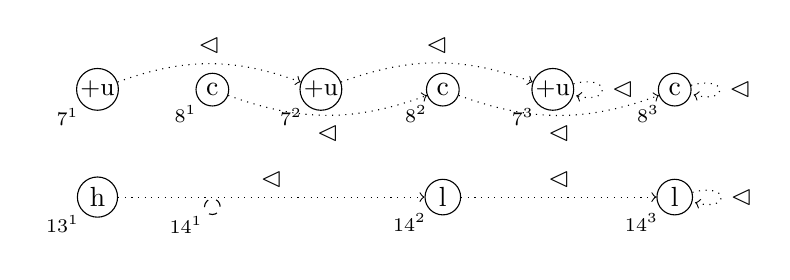
\begin{tikzpicture} [baseline = (z1.base)]
\matrix (m) [matrix of nodes, column sep = 1.5em, row sep = 1.5em]{
\node[draw,circle, inner sep =.5pt, label ={[label distance = -3pt] below left:\scriptsize$7^1$}](z1){\small +u}; & \node[draw,circle, inner sep =2pt, label ={[label distance = -3pt] below left:\scriptsize$8^1$}](z2){c}; & \node[draw,circle, inner sep =.5pt, label ={[label distance = -3pt] below left:\scriptsize$7^2$}](z11){\small +u}; & \node[draw,circle, inner sep =2pt, label ={[label distance = -3pt] below left:\scriptsize$8^2$}](z22){c}; & \node[draw,circle, inner sep =.5pt, label ={[label distance = -3pt] below left:\scriptsize$7^3$}](z111){\small +u}; & \node[draw,circle, inner sep =2pt, label ={[label distance = -3pt] below left:\scriptsize$8^3$}](z222){c}; \\
\node[draw,circle, inner sep =2pt, label ={[label distance = -3pt] below left:\scriptsize$13^1$}](t1){h}; &  \node[draw,circle, dashed, inner sep =2pt, label ={[label distance = -3pt] below left:\scriptsize$14^1$}](t2){\hspace{1em}}; & &  \node[draw,circle, inner sep =2pt, label ={[label distance = -3pt] below left:\scriptsize$14^2$}](t22){l}; & &  \node[draw,circle, inner sep =2pt, label ={[label distance = -3pt] below left:\scriptsize$14^3$}](t222){l}; \\
};
\path[->, dotted] (z1) edge[bend left=20] node[above,pos=.5]{$\vartriangleleft$}(z11); 
\path[->, dotted] (z11) edge[bend left=20] node[above,pos=.5]{$\vartriangleleft$}(z111); 
\path[->, dotted] (z2) edge[bend right=20] node[below,pos=.5]{$\vartriangleleft$}(z22); 
\path[->, dotted] (z22) edge[bend right=20] node[below,pos=.5]{$\vartriangleleft$}(z222); 
\path[->, dotted] (z111) edge[loop right] node{$\vartriangleleft$}(z111); 
\path[->, dotted] (z222) edge[loop right] node{$\vartriangleleft$}(z222); 
\draw[->, dotted] (t1) -- (t22) node[above, pos=.5]{$\vartriangleleft$};
\draw[->, dotted] (t22) -- (t222) node[above, pos=.5]{$\vartriangleleft$};
\path[->, dotted] (t222) edge[loop right] node{$\vartriangleleft$}(t222); 
\end{tikzpicture}
\end{center}\par
As mentioned above, Shanghai tone sandhi is well-studied among Chinese dialects. More recent acoustic evidence has cast some doubt on the veracity of the largely impressionistic claims that the contour of the first syllable spreads across the whole domain. \citet{Chen2008}, for example, provides evidence from a production study suggesting that all non-initial tones within a sandhi domain default to a [L] tone target instead of the rightmost tone on the first syllable. This, however, has no impact on its representability in our formalism. A transduction for this type of neutralization is nearly identical to the current analysis, with the only notable exception being in the definition of unary relations over tones; tones on first syllables are retained from the input in the first copy set, while all subsequent copies comprise a single [l] tone:
\begin{equation}
\begin{aligned}
P^{1}_{h}(x)&\myeq P_{h}(x)\land first(\delta(x)) & P^{2}_{h}(x)&\myeq\mathtt{False} & P^{3}_{h}(x)&\myeq\mathtt{False} \\
P^{1}_{l}(x)&\myeq P_{l}(x)\land first(\delta(x)) & P^{2}_{l}(x)&\myeq P_{t}(x)\land first(x) & P^{3}_{l}(x)&\myeq P_{t}(x)\land first(x) \\
\end{aligned}
\end{equation}
Crucial to our purposes here is the observation that both analyses of this process can be formalized as logical transductions using the same complexity class of logic (QF).
\section{Zhangping}
Zhangping is a Min dialect spoken in Fujian province \citep{Chen2000, Zhang1983}, and is reported as a case of widespread contrast neutralization; tones in non-final syllables revert to a default realization, regardless of input specification. We focus on a particular process which neutralizes register contrasts on non-final falling contours.
\begin{center}
\begin{tabular}[t]{lll}
\textipa{kin} & \textipa{tsai} & `nearby' \\
HM & MH & base form \\
ML & MH &  sandhi form \\
\hspace{1em} \\
tsi & giu & `freedom' \\
HM & ML & base form \\
ML & ML & sandhi form \\
\end{tabular}
\hspace{1cm}
\begin{tabular}[t]{lll}
\textipa{kin} & \textipa{tsiap} & `quickly' \\
ML & HM & base form \\
ML & HM &  sandhi form \\
\hspace{1em} \\
tsi & so & `sister-in-law' \\
ML & ML & base form \\
ML & ML & sandhi form \\
\end{tabular}
\end{center}
In the examples above, the contrast between segmentally-identical /HM/ and /ML/ contours neutralizes in non-final position within a word. This process is restricted to falling contour tones 53, 53q (checked tone), and 31.\par
We define a transduction $\tau$ over a Bao input signature to model this neutralization process in much the same way as dissimilation, that is, as a feature-changing operation. Crucial here are definitions of unary relations over register and terminal tonal nodes; we must restrict the process to forms with non-final falling contours, and ensure that the non-final syllable of the output is uniformly low-registered, but not derive any other changes. Definitions of syllable, root, and `c' node unary relations are consistent between input and output signatures, and are therefore omitted. The same is true for all binary functions: $\alpha(x)\ap y$, $\delta(x)\ap y$, and $succ(x)\ap y$.
\begin{equation}
\begin{aligned}
P^{\tau}_{+u}(x)&\myeq P_{+u}(x)\land final(x)  \\
P^{\tau}_{-u}(x)&\myeq P_{-u}(x) \lor (P_{+u}(x)\land \neg final(x)) \\
P^{\tau}_{l}(x)&\myeq \big(P_{l}(x)\land \neg final(\delta(x))\land final(\delta(succ(x)))\big)\,\lor \\
&\quad\,\,\big(P_{l}(x)\land final(\delta(x))\big) \\
P^{\tau}_{h}(x)&\myeq \big(P_{h}(x)\land\neg final(\delta(x))\land\neg final(\delta(succ(x)))\big)\,\lor \\
\end{aligned}
\end{equation}
In this process, non-final high-registered tones are changed to low register, while tones on final syllables (high or low) stay the same, as are underlyingly low-registered tones (via the definitions of $P_{+u}$ and $P_{-u}$). Among the tones which conform to these register specifications, only non-final falling contours undergo the feature-changing operation; non-final rising contours or level tones are exempt, as are any final tone. The definition of the transduction predicts neutralization only on tones of this type, and does not over-apply to other configurations.
\begin{center}
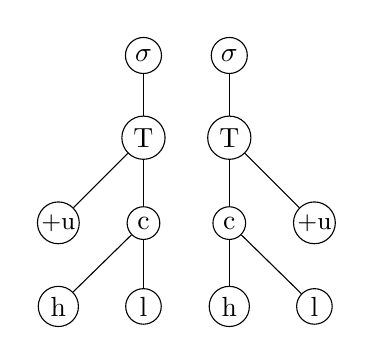
\begin{tikzpicture} [baseline = (y1.base)]
\matrix (m) [matrix of nodes, column sep = 1.5em, row sep = 1.5em]{
& \node[draw,circle, inner sep =2pt](x1){$\sigma$};  &  \node[draw,circle, inner sep =2pt](x2){$\sigma$};  \\
& \node[draw,circle, inner sep =2pt](y1){T}; &   \node[draw,circle, inner sep =2pt](y2){T}; \\
\node[draw,circle, inner sep =.5pt](z1){\small +u}; & \node[draw,circle, inner sep =2pt](z2){c}; &   \node[draw,circle, inner sep =2pt](z3){c}; & \node[draw,circle, inner sep =.5pt](z4){\small +u}; \\
\node[draw,circle, inner sep =2pt](t1){h}; & \node[draw,circle, inner sep =2pt](t2){l}; &  \node[draw,circle, inner sep =2pt](t3){h}; & \node[draw,circle, inner sep =2pt](t4){l}; \\
};
\draw (x1) -- (y1);
\draw (x2) -- (y2);
\draw (z1) -- (y1);
\draw (z2) -- (y1);
\draw (z2) -- (t1);
\draw (z2) -- (t2);
\draw (y2) -- (z3);
\draw (y2) -- (z4);
\draw (z3) -- (t3);
\draw (t4) -- (z3);
\end{tikzpicture}
\hspace{.3cm}
$\mapsto$
\hspace{.3cm}
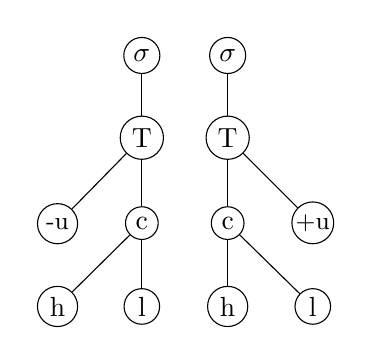
\begin{tikzpicture} [baseline = (y1.base)]
\matrix (m) [matrix of nodes, column sep = 1.5em, row sep = 1.5em]{
& \node[draw,circle, inner sep =2pt](x1){$\sigma$};  &  \node[draw,circle, inner sep =2pt](x2){$\sigma$};  \\
& \node[draw,circle, inner sep =2pt](y1){T}; &   \node[draw,circle, inner sep =2pt](y2){T}; \\
\node[draw,circle, inner sep =2pt](z1){\small -u}; & \node[draw,circle, inner sep =2pt](z2){c}; &   \node[draw,circle, inner sep =2pt](z3){c}; & \node[draw,circle, inner sep =.5pt](z4){\small +u}; \\
\node[draw,circle, inner sep =2pt](t1){h}; & \node[draw,circle, inner sep =2pt](t2){l}; &  \node[draw,circle, inner sep =2pt](t3){h}; & \node[draw,circle, inner sep =2pt](t4){l}; \\
};
\draw (x1) -- (y1);
\draw (x2) -- (y2);
\draw (z1) -- (y1);
\draw (z2) -- (y1);
\draw (z2) -- (t1);
\draw (z2) -- (t2);
\draw (y2) -- (z3);
\draw (y2) -- (z4);
\draw (z3) -- (t3);
\draw (t4) -- (z3);
\end{tikzpicture}
\hspace{.3cm}
$\equiv$ /HM.HM/$\mapsto$[ML.HM]
\end{center}
\begin{center}
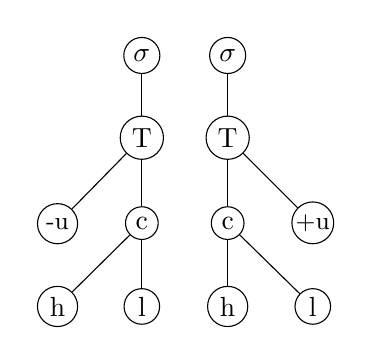
\begin{tikzpicture} [baseline = (y1.base)]
\matrix (m) [matrix of nodes, column sep = 1.5em, row sep = 1.5em]{
& \node[draw,circle, inner sep =2pt](x1){$\sigma$};  &  \node[draw,circle, inner sep =2pt](x2){$\sigma$};  \\
& \node[draw,circle, inner sep =2pt](y1){T}; &   \node[draw,circle, inner sep =2pt](y2){T}; \\
\node[draw,circle, inner sep =2pt](z1){\small -u}; & \node[draw,circle, inner sep =2pt](z2){c}; &   \node[draw,circle, inner sep =2pt](z3){c}; & \node[draw,circle, inner sep =.5pt](z4){\small +u}; \\
\node[draw,circle, inner sep =2pt](t1){h}; & \node[draw,circle, inner sep =2pt](t2){l}; &  \node[draw,circle, inner sep =2pt](t3){h}; & \node[draw,circle, inner sep =2pt](t4){l}; \\
};
\draw (x1) -- (y1);
\draw (x2) -- (y2);
\draw (z1) -- (y1);
\draw (z2) -- (y1);
\draw (z2) -- (t1);
\draw (z2) -- (t2);
\draw (y2) -- (z3);
\draw (y2) -- (z4);
\draw (z3) -- (t3);
\draw (t4) -- (z3);
\end{tikzpicture}
\hspace{.3cm}
$\mapsto$
\hspace{.3cm}
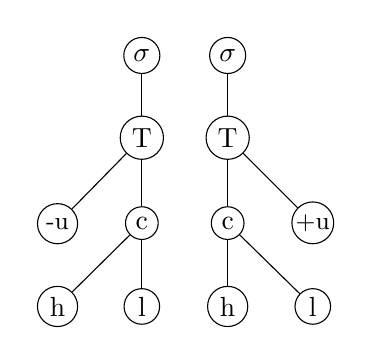
\begin{tikzpicture} [baseline = (y1.base)]
\matrix (m) [matrix of nodes, column sep = 1.5em, row sep = 1.5em]{
& \node[draw,circle, inner sep =2pt](x1){$\sigma$};  &  \node[draw,circle, inner sep =2pt](x2){$\sigma$};  \\
& \node[draw,circle, inner sep =2pt](y1){T}; &   \node[draw,circle, inner sep =2pt](y2){T}; \\
\node[draw,circle, inner sep =2pt](z1){\small -u}; & \node[draw,circle, inner sep =2pt](z2){c}; &   \node[draw,circle, inner sep =2pt](z3){c}; & \node[draw,circle, inner sep =.5pt](z4){\small +u}; \\
\node[draw,circle, inner sep =2pt](t1){h}; & \node[draw,circle, inner sep =2pt](t2){l}; &  \node[draw,circle, inner sep =2pt](t3){h}; & \node[draw,circle, inner sep =2pt](t4){l}; \\
};
\draw (x1) -- (y1);
\draw (x2) -- (y2);
\draw (z1) -- (y1);
\draw (z2) -- (y1);
\draw (z2) -- (t1);
\draw (z2) -- (t2);
\draw (y2) -- (z3);
\draw (y2) -- (z4);
\draw (z3) -- (t3);
\draw (t4) -- (z3);
\end{tikzpicture}
\hspace{.3cm}
$\equiv$ /ML.HM/$\mapsto$[ML.HM]
\end{center}
\begin{center}
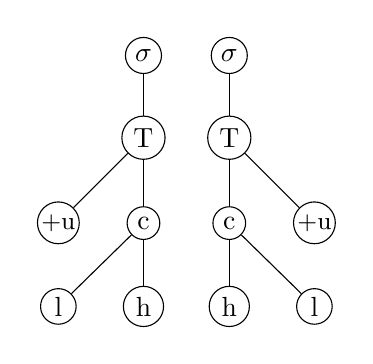
\begin{tikzpicture} [baseline = (y1.base)]
\matrix (m) [matrix of nodes, column sep = 1.5em, row sep = 1.5em]{
& \node[draw,circle, inner sep =2pt](x1){$\sigma$};  &  \node[draw,circle, inner sep =2pt](x2){$\sigma$};  \\
& \node[draw,circle, inner sep =2pt](y1){T}; &   \node[draw,circle, inner sep =2pt](y2){T}; \\
\node[draw,circle, inner sep =.5pt](z1){\small +u}; & \node[draw,circle, inner sep =2pt](z2){c}; &   \node[draw,circle, inner sep =2pt](z3){c}; & \node[draw,circle, inner sep =.5pt](z4){\small +u}; \\
\node[draw,circle, inner sep =2pt](t1){l}; & \node[draw,circle, inner sep =2pt](t2){h}; &  \node[draw,circle, inner sep =2pt](t3){h}; & \node[draw,circle, inner sep =2pt](t4){l}; \\
};
\draw (x1) -- (y1);
\draw (x2) -- (y2);
\draw (z1) -- (y1);
\draw (z2) -- (y1);
\draw (z2) -- (t1);
\draw (z2) -- (t2);
\draw (y2) -- (z3);
\draw (y2) -- (z4);
\draw (z3) -- (t3);
\draw (t4) -- (z3);
\end{tikzpicture}
\hspace{.3cm}
$\not\mapsto$
\hspace{.3cm}
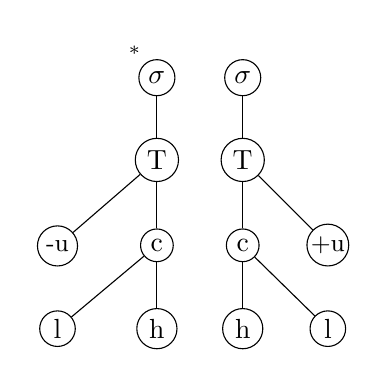
\begin{tikzpicture} [baseline = (y1.base)]
\matrix (m) [matrix of nodes, column sep = 1.5em, row sep = 1.5em]{
& \node[draw,circle, inner sep =2pt, label={[label distance=-3pt] above left:\scriptsize *}](x1){$\sigma$};  &  \node[draw,circle, inner sep =2pt](x2){$\sigma$};  \\
& \node[draw,circle, inner sep =2pt](y1){T}; &   \node[draw,circle, inner sep =2pt](y2){T}; \\
\node[draw,circle, inner sep =2pt](z1){\small -u}; & \node[draw,circle, inner sep =2pt](z2){c}; &   \node[draw,circle, inner sep =2pt](z3){c}; & \node[draw,circle, inner sep =.5pt](z4){\small +u}; \\
\node[draw,circle, inner sep =2pt](t1){l}; & \node[draw,circle, inner sep =2pt](t2){h}; &  \node[draw,circle, inner sep =2pt](t3){h}; & \node[draw,circle, inner sep =2pt](t4){l}; \\
};
\draw (x1) -- (y1);
\draw (x2) -- (y2);
\draw (z1) -- (y1);
\draw (z2) -- (y1);
\draw (z2) -- (t1);
\draw (z2) -- (t2);
\draw (y2) -- (z3);
\draw (y2) -- (z4);
\draw (z3) -- (t3);
\draw (t4) -- (z3);
\end{tikzpicture}
\hspace{.3cm}
$\equiv$ /MH.HM/$\not\mapsto$*[LM.HM]
\end{center}
\begin{center}
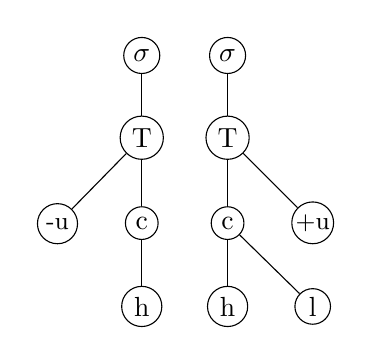
\begin{tikzpicture} [baseline = (y1.base)]
\matrix (m) [matrix of nodes, column sep = 1.5em, row sep = 1.5em]{
& \node[draw,circle, inner sep =2pt](x1){$\sigma$};  &  \node[draw,circle, inner sep =2pt](x2){$\sigma$};  \\
& \node[draw,circle, inner sep =2pt](y1){T}; &   \node[draw,circle, inner sep =2pt](y2){T}; \\
\node[draw,circle, inner sep =2pt](z1){\small -u}; & \node[draw,circle, inner sep =2pt](z2){c}; &   \node[draw,circle, inner sep =2pt](z3){c}; & \node[draw,circle, inner sep =.5pt](z4){\small +u}; \\
& \node[draw,circle, inner sep =2pt](t2){h}; &  \node[draw,circle, inner sep =2pt](t3){h}; & \node[draw,circle, inner sep =2pt](t4){l}; \\
};
\draw (x1) -- (y1);
\draw (x2) -- (y2);
\draw (z1) -- (y1);
\draw (z2) -- (y1);
\draw (z2) -- (t2);
\draw (y2) -- (z3);
\draw (y2) -- (z4);
\draw (z3) -- (t3);
\draw (t4) -- (z3);
\end{tikzpicture}
\hspace{.3cm}
$\not\mapsto$
\hspace{.3cm}
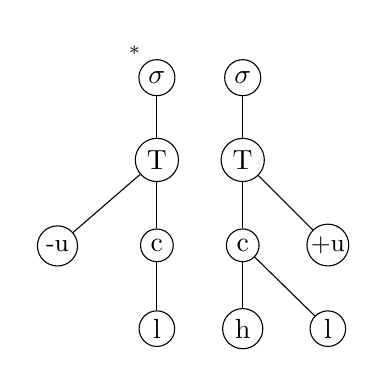
\begin{tikzpicture} [baseline = (y1.base)]
\matrix (m) [matrix of nodes, column sep = 1.5em, row sep = 1.5em]{
& \node[draw,circle, inner sep =2pt, label={[label distance=-3pt] above left:\scriptsize *}](x1){$\sigma$};  &  \node[draw,circle, inner sep =2pt](x2){$\sigma$};  \\
& \node[draw,circle, inner sep =2pt](y1){T}; &   \node[draw,circle, inner sep =2pt](y2){T}; \\
\node[draw,circle, inner sep =2pt](z1){\small -u}; & \node[draw,circle, inner sep =2pt](z2){c}; &   \node[draw,circle, inner sep =2pt](z3){c}; & \node[draw,circle, inner sep =.5pt](z4){\small +u}; \\
& \node[draw,circle, inner sep =2pt](t2){l}; &  \node[draw,circle, inner sep =2pt](t3){h}; & \node[draw,circle, inner sep =2pt](t4){l}; \\
};
\draw (x1) -- (y1);
\draw (x2) -- (y2);
\draw (z1) -- (y1);
\draw (z2) -- (y1);
\draw (z2) -- (t2);
\draw (y2) -- (z3);
\draw (y2) -- (z4);
\draw (z3) -- (t3);
\draw (t4) -- (z3);
\end{tikzpicture}
\hspace{.3cm}
$\equiv$ /M.HM/$\not\mapsto$*[L.HM]
\end{center}
The definition of the transduction will only evaluate to true for maps with a non-final, high-falling contour in the domain and a non-final, low-falling contour in the codomain, or a non-final low-falling contour in both (for which it will be vacuously true). Crucially, it will not evaluate to true for inputs with non-final high-rising contours which surface as low-rising contours, nor for input high level tones which surface as low level tones. In other words, the transduction as defined does not overgenerate.
\bibliographystyle{apalike}
\bibliography{references}
\end{document}